\documentclass{../lab_class}

\usepackage{fancyhdr}
\pagestyle{fancy}
\rhead{П.\,Ю. Смирнов, 687 гр.}
\lhead{Лабораторная работа № 4.7.3, МФТИ, весна 2018}

\begin{document}

{\Large 4.7.3 -- Поляризация.}

\paragraph{Цель работы.}
Ознакомление с методами получения и анализа поляризованного света.

В работе используются: оптическая скамья с осветителем; зелёный светофильтр; два поляроида; чёрное зеркало; полированная эбонитовая пластинка; стопа стеклянных пластинок; слюдяные пластинки разной толщины; пластинки в 1/4 и 1/2 длины волны; пластинка в одну длину волны для зелёного света (пластинка чувствительного оттенка).

Особенность данной работы -- качественный, описательный характер.

\paragraph{Теоретическая часть.}
\begin{wrapfigure}{r}{0.3\textwidth}
  \vspace{-20pt}
  \begin{center}
    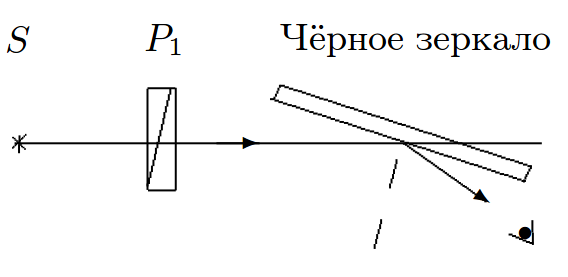
\includegraphics[width=0.28\textwidth]{01.png}
  \end{center}
  \vspace{-20pt}
  \caption{Определение разрешённого направления поляроида.}
  \label{fig:scheme01}
  \vspace{-10pt}
\end{wrapfigure}

Электромагнитные волны, как следует из уравнений Максвелла, поперечны; потому волну можно охарактеризовать тремя векторами -- волновым вектором (перенос энергии, распространение волны), амплитудным (направление колебаний напряженности поля) и поляризационным -- вращение амплитудного вектора в плоскости колебаний. В случае монохроматической волны компоненты вектора напряженности поля меняются в плоскости колебаний по гармоническому закону; отсюда (a la фигуры Лиссажу) следует, что траектория конца амплитудного вектора есть эллипс (\emph{эллиптическая поляризация}). Важные частные случаи, которые нас будут интересовать -- круговая и линейная поляризация. В последнем случае волну называют также \emph{плоско-поляризованной}, поскольку амплитудный вектор колеблется в одной плоскости. 

Также часто встречаются такие понятия, как $s$-поляризованная и $p$-поляризованная волны. В первом случае вектор напряженности электрического поля перпендикулярен плоскости падения, во втором -- лежит в ней. Интерес в такой классификации состоит в том, что, как следует из формул Френеля, при угле падения \emph{Брюстера} $\varphi_B = \arctan n$ отраженный свет является полностью ($s$) поляризованным.

\paragraph{Разрешенное направление поляроида. Определение показателя преломления.}
Схема установки приведена на рис. \ref{fig:scheme01}. Отражённый от чёрного зеркала свет имеет минимальную интенсивность в том случае, если угол падения есть угол Брюстера и в падающем пучке вектор $E$ лежит в плоскости падения -- так мы определим разрешенное направления поляроида, и, коль мы знаем при этом и угол Брюстера, и показатель преломления пластины, играющей роль зеркала.

В нашей работы мы измеряем разрешенное направление двух поляроидов $P_1$ и $P_2$ и угол Брюстера для эбонитовой пластины (со светофильтром и без):
\begin{gather*}
	\varphi_{P_1} = 30^{\circ},  \\
	\varphi_{P_2} = 103^{\circ}, \\
	\varphi_{Br} = 49^{\circ}, \\
	\varphi_{Br_{filter}} = 45^{\circ}.
\end{gather*}

Со светофильтром получилось хуже. Из выражения для угла Брюстера отсюда получаем оценку показателя преломления эбонита: $\boxed{n \simeq 1.18}$. Табличное -- 1.8. Проблема в том, определение интенсивности <<на глаз>> -- не лучшая идея.

\pagebreak

\paragraph{Эллиптически поляризованный свет.}
\begin{wrapfigure}{r}{0.3\textwidth}
  \vspace{-20pt}
  \begin{center}
    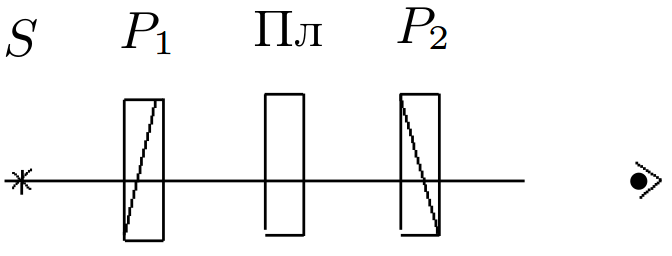
\includegraphics[width=0.28\textwidth]{02.png}
  \end{center}
  \vspace{-20pt}
  \caption{Исследуем двоякопреломляющую пластинку!}
  \label{fig:scheme02}
  \vspace{-10pt}
\end{wrapfigure}

Эллиптически поляризованный свет можно получить из линейно поляризованного, используя двоякопреломляющие кристаллические пластинки. Показатель преломления в них задаётся тензором диэлектрической проницаемости; он симметричен, потому ему можно поставить в соответствие эллипсоид проницаемости. Его оси называют \emph{главными направлениями} -- свет вдоль них распространяется с разной скоростью, не меняя своей поляризации.

Пусть теперь на пластинку падает линейно поляризованная волна. Её можно разложить вдоль главных (перпендикулярных) направлений; поскольку скорость по ним различна, на выходе мы получим суперпозицию двух уже \emph{несинфазных} волн -- иными словами, эллиптическую поляризацию. Разность фаз есть $\Delta \varphi = k d (n_x - n_y)$, где $d$ -- толщина пластинки. Ясно, что при $d = \lambda$ мы получим сдвиг фаз $2 \pi$ -- ничего не изменится; при $d = \lambda / 2$ -- сдвиг фаз $\pi$, поляризация по-прежнему линейная, но имеет противоположное направление; наконец, при $d = \lambda / 4$ мы получаем сдвиг фаз $\pi/2$ и эллиптическую поляризацию.

У нас есть две пластинки. Определим их главные направления -- для этого поставим каждую из них (рис. \ref{fig:scheme02}) между скрещеными поляроидами и будем крутить до тех пор, пока главное направление не совпадет с разрешенным направлением поляриода $P_2$. Получаем:

\begin{gather*}
	\varphi_1 = 64^{\circ}, \\
	\varphi_2 = 80^{\circ}.
\end{gather*}
Заметим, что направления, очевидно, чередуются каждые $\pi/2$ радиан.

\begin{wrapfigure}{l}{0.3\textwidth}
  \vspace{-20pt}
  \begin{center}
    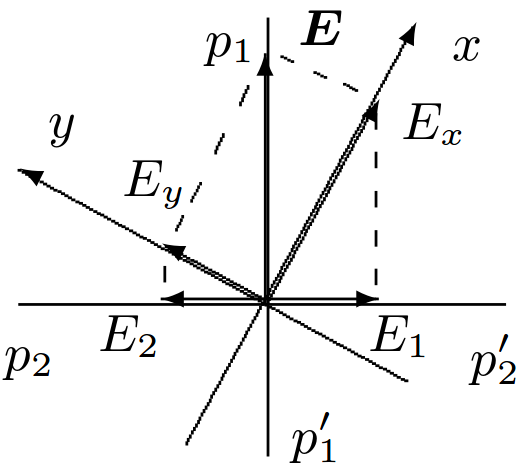
\includegraphics[width=0.28\textwidth]{03.png}
  \end{center}
  \vspace{-20pt}
  \caption{К объяснению интерференции поляризованных лучей.}
  \label{fig:scheme03}
  \vspace{-10pt}
\end{wrapfigure}

В нашей работе одна из пластинок имеет толщину $\lambda/2$, другая -- $\lambda/4$. Используя высказанные выше соображения о поляризации света, прошедшего пластинку, мы без труда (исп. также поляризатор) определяем, что первая пластинка имеет линейную поляризацию (соотв. $\lambda/2$), вторая -- круговую (соотв. $\lambda/4$).

Пластинкой \emph{чувствительного оттенка} называют пластинку в форме стрелки (вдоль неё -- быстрое главное направление) для зелёной спектральной компоненты. С её помощью мы можем определить <<быстрое>> и <<медленное>> главные направления пластинки в $\lambda/4$. Если расположить пластинки так, чтобы их главные быстрые направления совпали, то разность хода $E_x$ и $E_y$ составит уже $5 \lambda/4$, что соответствует более красному свету; потому при освещении белым пучком погасится красная часть спектра, пластинка будет казаться зеленовато-голубой. Если же названные направления будут перпендикулярны, то цвет будет фиолетово-голубой.

Двоякопреломляющая в скрещенных поляризаторах, как кажется, меняет цвет. Это можно объяснить интерференцией поляризованных лучей. На рис. \ref{fig:scheme03} $p_1$ соотв. первому поляроиду, $p_2$ -- второму (разрешенные направления), $x,y$ -- главные направления пластинки. На выходе из пластинки волны имеют сдвиг фаз, соотв. интерферируют; отношение амплитуд и сдвиг фаз не меняется при повороте пластинки. Дополнительный фазовые сдвиг можно получить, вращая второй поляроид.

\paragraph{Вывод.}
В данной работе мы описали кратко способ получения и анализа поляризованного света, а также оговорили отдельные значимые в данном контексте вопросы кристаллооптики.

\end{document}